\documentclass[conference]{IEEEtran}
\usepackage[utf8]{inputenc}
\usepackage[vietnamese]{babel}
\usepackage{amsmath,amssymb,amsfonts}
\usepackage{algorithmic}
\usepackage{graphicx}
\usepackage{textcomp}
\usepackage{xcolor}
\usepackage{booktabs}
\usepackage{url}
\usepackage{listings}

\lstset{
  basicstyle=\footnotesize\ttfamily,
  breaklines=true,
  frame=single,
  columns=fullflexible
}

\begin{document}

\title{Tự Động Hóa Sinh và Đánh Giá Trò Chơi Giáo Dục Tương Tác Văn Bản Tiếng Việt Quy Mô Lớn Sử Dụng Mô Hình Ngôn Ngữ Lớn và Ngôn Ngữ Kịch Bản Ink}

\author{\IEEEauthorblockN{Nguyễn Hoàng Hải}
\IEEEauthorblockA{\textit{Khoa Công nghệ Đa phương tiện} \\
\textit{Học viện Công nghệ Bưu chính Viễn thông}\\
Hà Nội, Việt Nam \\
nghoanghaihn@gmail.com}
\and
\IEEEauthorblockN{Đỗ Ngọc Thiện}
\IEEEauthorblockA{\textit{Khoa Công nghệ Đa phương tiện} \\
\textit{Học viện Công nghệ Bưu chính Viễn thông}\\
Hà Nội, Việt Nam \\
dongocthien1411@gmail.com}
}

\maketitle

\begin{abstract}
Thiết kế trò chơi giáo dục (Educational Serious Games) phục vụ giáo dục thường đòi hỏi chi phí sản xuất cao và kỹ năng lập trình chuyên sâu, tạo nên rào cản kỹ thuật đáng kể đối với phần lớn giáo viên và các nhà sư phạm. Nghiên cứu này trình bày việc bản địa hóa, mở rộng và hoàn thiện hệ thống SINE-VN (Serious Interactive Narrative Engine for Vietnamese), tự động hóa hoàn toàn quy trình chuyển đổi các bộ đề thi trắc nghiệm tĩnh quy mô lớn (lên tới 40--50 câu hỏi) sang các trò chơi giáo dục tương tác văn bản (Interactive Fiction Serious Games - IF-SG) bằng Tiếng Việt. Hệ thống tích hợp mô hình ngôn ngữ lớn nguồn mở họ Qwen 2.5 cùng ngôn ngữ kịch bản chuyên dụng Ink. Nghiên cứu đóng góp: (1) Kiến trúc đa hồi ghép nối tất định (Multi-Stage Stitched Architecture) giải quyết triệt để giới hạn tràn bộ đệm token và suy thoái ngữ cảnh khi sinh các bộ đề thi dài; (2) Cơ chế tự khử trùng lặp không gian tên phân cảnh (\texttt{deduplicate\_knots}); (3) Cải tiến đột phá cấu trúc lựa chọn vĩnh viễn (Sticky Choices \texttt{+}) triệt tiêu hoàn toàn lỗi cạn kiệt nhánh trạng thái khi người học chọn sai nhiều lần; và (4) Bộ trích xuất đề thi đa thể thức (Word/PDF) bảo toàn nguyên vẹn công thức MathType/OMML, ký hiệu hóa học, dấu typographic và ngữ cảnh hội thoại. Thực nghiệm toàn diện trên 5 môn thi Tốt nghiệp THPT Quốc gia (Toán học, Hóa học 40 câu, Vật lý 40 câu, Tiếng Anh 50 câu, Địa lý 24 câu) chứng minh hệ thống đạt tỷ lệ biên dịch, khả năng chơi toàn vẹn và độ trung thực học thuật tuyệt đối 100\% ($S = C \cdot P \cdot Q = 1$), mở ra bước đột phá cho ứng dụng AI tạo sinh vào công nghệ giáo dục tại Việt Nam.
\end{abstract}

\begin{IEEEkeywords}
trò chơi giáo dục; kịch bản tương tác văn bản; mô hình ngôn ngữ lớn; hệ thống SINE-VN; ngôn ngữ kịch bản Ink; kiến trúc đa hồi ghép nối; công nghệ giáo dục.
\end{IEEEkeywords}

\section{GIỚI THIỆU}
Trò chơi giáo dục (Serious Games) đóng vai trò là công cụ đột phá thúc đẩy chuyển đổi số và nâng cao chất lượng giáo dục hiện đại \cite{rogosch2026}. Khác với các trò chơi giải trí thuần túy, trò chơi giáo dục tích hợp chặt chẽ các mục tiêu sư phạm vào cơ chế tương tác, tạo nên môi trường học tập kích thích sự tò mò, khám phá và tăng cường phản hồi nhận thức theo thời gian thực \cite{connolly2012}. Nhiều nghiên cứu thực nghiệm đã chứng minh rằng hình thức học tập dựa trên trò chơi (Game-Based Learning) giúp gia tăng đáng kể mức độ gắn kết của học sinh, cải thiện khả năng ghi nhớ thông tin dài hạn và nuôi dưỡng tư duy giải quyết vấn đề độc lập \cite{horn2025}.

Mặc dù mang lại hiệu quả sư phạm vượt trội, việc triển khai trò chơi giáo dục trên diện rộng trong nhà trường vẫn vấp phải một rào cản kỹ thuật nghiêm trọng, được định nghĩa là ``nút thắt cổ chai tác giả'' (Authoring Bottleneck) \cite{horn2025}. Phần lớn giáo viên và các chuyên gia giáo dục sở hữu năng lực sư phạm chuyên sâu nhưng lại hạn chế về kỹ năng lập trình phần mềm và thiết kế trò chơi (Game Design). Quy trình sản xuất một trò chơi học tập tương tác truyền thống thường đòi hỏi sự phối hợp liên ngành phức tạp giữa biên kịch, lập trình viên và họa sĩ đồ họa, tiêu tốn từ vài tuần đến nhiều tháng với kinh phí đầu tư vượt quá khả năng tài chính của đa số cơ sở giáo dục phổ thông.

Sự bùng nổ của Trí tuệ Nhân tạo Tạo sinh (Generative AI), tiêu biểu là các Mô hình Ngôn ngữ Lớn (LLMs), đã mở ra triển vọng tự động hóa hoàn toàn quy trình thiết kế nội dung trò chơi \cite{gallotta2024}. Nhờ khả năng phân tích ngôn ngữ tự nhiên và sinh mã kịch bản, LLM có thể đóng vai trò như một trợ lý thiết kế ảo, chuyển hóa nhanh chóng các ngân hàng câu hỏi kiến thức thành các kịch bản tương tác phong phú. Tuy nhiên, khi ứng dụng trực tiếp LLM vào việc sinh mã kịch bản trò chơi quy mô lớn, các công trình đi trước như STORY2GAME \cite{zhou2025}, GENEVA \cite{leandro2024} và ngay cả khung SINE nguyên bản của Rogosch và Schrader (2026) \cite{rogosch2026} đều chỉ dừng lại ở các bài kiểm tra quy mô vi mô (2 đến 5 câu hỏi, tối đa 10 câu). Khi mở rộng lên quy mô đề thi thực tế (40 đến 50 câu hỏi), các hệ thống này đối mặt với bốn thách thức học thuật và kỹ thuật nghiêm trọng:
\begin{enumerate}
    \item \textit{Tràn giới hạn token và suy thoái ngữ cảnh (Token Ceiling \& Context Drift):} Một kịch bản game hoàn chỉnh cho đề thi 40--50 câu đòi hỏi từ 600 đến 800+ dòng mã Ink phức tạp với hàng trăm phân cảnh và nhánh rẽ. LLM sinh đơn khối (Monolithic generation) tất yếu bị cạn kiệt bộ đệm output token (thường đứt gãy ở câu 35--43), sinh mã dang dở dẫn đến lỗi cú pháp nghiêm trọng.
    \item \textit{Xung đột không gian tên phân cảnh (Namespace Collisions):} Khi chia nhỏ kịch bản để sinh từng phần hoặc khi mô hình lặp lại các nút thắt chuyển tiếp (ví dụ: \texttt{=== act\_2\_start ===}), trình biên dịch Ink sẽ báo lỗi dừng biên dịch do trùng lặp dòng chảy (\textit{Duplicate flow error}).
    \item \textit{Cạn kiệt nhánh trạng thái (Choice Exhaustion):} Việc sử dụng toán tử lựa chọn tiêu hao (\texttt{*}) khiến kịch bản bị xóa phương án sai sau khi chọn, dẫn đến ngõ cụt hoàn toàn nếu học sinh thử lại nhiều lần, phá vỡ tính chơi được ($P = 0$).
    \item \textit{Mất mát biểu thức và ký hiệu chuyên ngành:} Các đề thi Khoa học Tự nhiên (Hóa học, Vật lý, Toán học) và Ngoại ngữ chứa mật độ dày đặc công thức MathType/OMML, chỉ số hóa học ($Al_2(SO_4)_3$), ký hiệu Hy Lạp, dấu typographic thông minh và hội thoại nhiều nhân vật. Bộ trích xuất văn bản thô sơ thường làm biến dạng ký hiệu hoặc gây lỗi phân tích JSON do dấu ngoặc kép chưa escape.
\end{enumerate}

Nhằm giải quyết triệt để các rào cản trên, nghiên cứu này phát triển và hoàn thiện hệ thống SINE-VN, đưa năng lực tự động hóa sinh trò chơi giáo dục lên quy mô đề thi chuẩn quốc gia. Bài báo đóng góp năm nội dung khoa học và kỹ thuật trọng tâm:
\begin{enumerate}
    \item \textit{Kiến trúc Đa Hồi Ghép Nối Tất Định (Multi-Stage Stitched Architecture):} Cơ chế tự động phân đoạn các đề thi quy mô lớn ($>12$ câu hỏi) thành các hồi nối tiếp tuần tự, sinh mã cục bộ có kiểm soát ngữ cảnh và ghép nối tất định bằng thuật toán định tuyến đồ thị bảo đảm tính kết nối toàn vẹn ($P = 1$).
    \item \textit{Thuật toán Khử trùng lặp và Tự lành Cú pháp (\texttt{deduplicate\_knots}):} Quét AST và xử lý xung đột không gian tên giữa các phân cảnh hồi, đồng thời chuẩn hóa đóng ngoặc lựa chọn (\texttt{+ [Option] ->}) triệt tiêu lỗi treo giao diện Web (Black Screen UI freeze).
    \item \textit{Cải tiến đột phá cú pháp Sticky Choice (\texttt{+}):} Triệt tiêu hoàn toàn lỗ hổng cạn kiệt nhánh trạng thái trong Ink, thiết lập chu trình tự sửa lỗi sư phạm bền vững cho người học.
    \item \textit{Động cơ trích xuất đề thi chuyên sâu đa thể thức:} Tích hợp tự động hóa Microsoft Word COM, trích xuất nguyên vẹn công thức MathType/OMML, chỉ số hóa học, bảo toàn nguyên vẹn lời thoại nhân vật trong đề Ngoại ngữ và tự sửa lỗi JSON bằng \texttt{json-repair}.
    \item \textit{Thực nghiệm toàn diện trên 5 môn thi Tốt nghiệp THPT Quốc gia:} Đánh giá trên các bộ đề thi chính thức năm 2023 của Bộ Giáo dục và Đào tạo (Toán học, Hóa học 40 câu, Vật lý 40 câu, Tiếng Anh 50 câu, Địa lý 24 câu), chứng minh hệ thống đạt tỷ lệ thành công 100\% ở cả 3 tiêu chí $C \cdot P \cdot Q$.
\end{enumerate}

\section{CƠ SỞ LÝ THUYẾT VÀ TỔNG QUAN NGHIÊN CỨU}
\subsection{Trò chơi Tương tác Văn bản Giáo dục (IF-SG) và Ngôn ngữ Ink}
Trò chơi tương tác văn bản (Interactive Fiction - IF) là một thể loại trò chơi phiêu lưu dựa trên văn bản, nơi thế giới ảo, bối cảnh và hành vi của nhân vật được mô tả bằng ngôn ngữ tự nhiên, còn người chơi tương tác thông qua các lựa chọn phân nhánh \cite{riedl2013}. Trong nghiên cứu về AI và giáo dục, IF được coi là không gian trừu tượng lý tưởng vì loại bỏ được sự phức tạp của cơ chế vật lý và dựng hình 3D, từ đó tập trung tối đa nguồn lực tính toán vào cấu trúc dẫn dắt câu chuyện và kiểm tra năng lực tư duy của người học \cite{rogosch2026}.

Để mô hình hóa kịch bản IF có cấu trúc, ngôn ngữ Ink do Inkle Studios phát triển \cite{ink2025} hiện là chuẩn mực công nghiệp phổ biến nhất. Một tệp kịch bản Ink bao gồm ba thành phần cơ bản:
\begin{itemize}
    \item \textbf{Knots:} Các phân cảnh câu chuyện độc lập, được khai báo theo cú pháp \texttt{=== ten\_knot ===}.
    \item \textbf{Diverts:} Lệnh chuyển hướng trạng thái tức thời, ký hiệu bằng mũi tên \texttt{->}.
    \item \textbf{Choices:} Các nhánh tương tác dành cho người chơi. Ngôn ngữ Ink phân biệt hai toán tử: toán tử dấu sao \texttt{*} là lựa chọn tiêu hao (Transient Choice, biến mất sau khi chọn), và toán tử dấu cộng \texttt{+} là lựa chọn vĩnh viễn (Sticky Choice, hiển thị lại mỗi khi phân cảnh được tái truy cập).
\end{itemize}

\subsection{Ứng dụng LLM trong Thiết kế Trò chơi Tự động}
Nghiên cứu tổng quan của Gallotta et al. (2024) \cite{gallotta2024} đã phân loại các vai trò của LLM trong phát triển trò chơi: Game Master, Automated Designer, và NPC thông minh. Zhou et al. (2025) công bố hệ thống STORY2GAME \cite{zhou2025}, dịch cốt truyện phiêu lưu thành mã Python, nhưng chỉ giới hạn ở trò chơi giải trí mở. Tanaka và Simo-Serra (2024) \cite{tanaka2024} ứng dụng ngữ pháp GBNF để sinh luật trò chơi Ludii, nâng tỷ lệ phân tích cú pháp từ 23\% lên 68\% nhưng không kiểm soát được tính đúng đắn ngữ nghĩa. Leandro et al. (2024) với GENEVA \cite{leandro2024} và Farrell \& Ware (2025) \cite{farrell2025} đều nhấn mạnh rằng khi quy mô kịch bản vượt quá 10 bước, đồ thị cốt truyện sinh bởi LLM có xu hướng gãy vụn và mất định hướng.

\subsection{Khung Hệ thống SINE Nguyên bản và Rào cản Mở rộng}
Hệ thống SINE do Rogosch và Schrader (2026) \cite{rogosch2026} đề xuất là công trình tiên phong thiết lập quy trình sinh trò chơi giáo dục có kiểm thử tự động khép kín ($C \cdot P \cdot Q$) và tác tử tự sửa lỗi. Tuy nhiên, SINE nguyên bản bộc lộ các hạn chế căn bản khi triển khai thực tế:
\begin{enumerate}
    \item Chỉ thử nghiệm trên tiếng Anh và các bài kiểm tra ngắn (2--5 câu hỏi).
    \item Sử dụng toán tử tiêu hao \texttt{*}, gây đứt gãy đồ thị ($P = 0$) trong các chu trình học tập thử lại.
    \item Thiếu hoàn toàn cơ chế chia phân đoạn đa hồi, dẫn đến việc LLM không thể sinh được các đề thi chuẩn 40--50 câu.
    \item Không có khả năng trích xuất công thức toán học và ký hiệu khoa học từ các tệp đề thi Word/PDF thực tế.
\end{enumerate}

\section{KIẾN TRÚC HỆ THỐNG SINE-VN ĐỀ XUẤT}
Hệ thống SINE-VN được thiết kế theo kiến trúc đường ống tự động hóa toàn trình khép kín, được minh họa chi tiết tại Hình \ref{fig:arch}.

\begin{figure}[htbp]
\centering
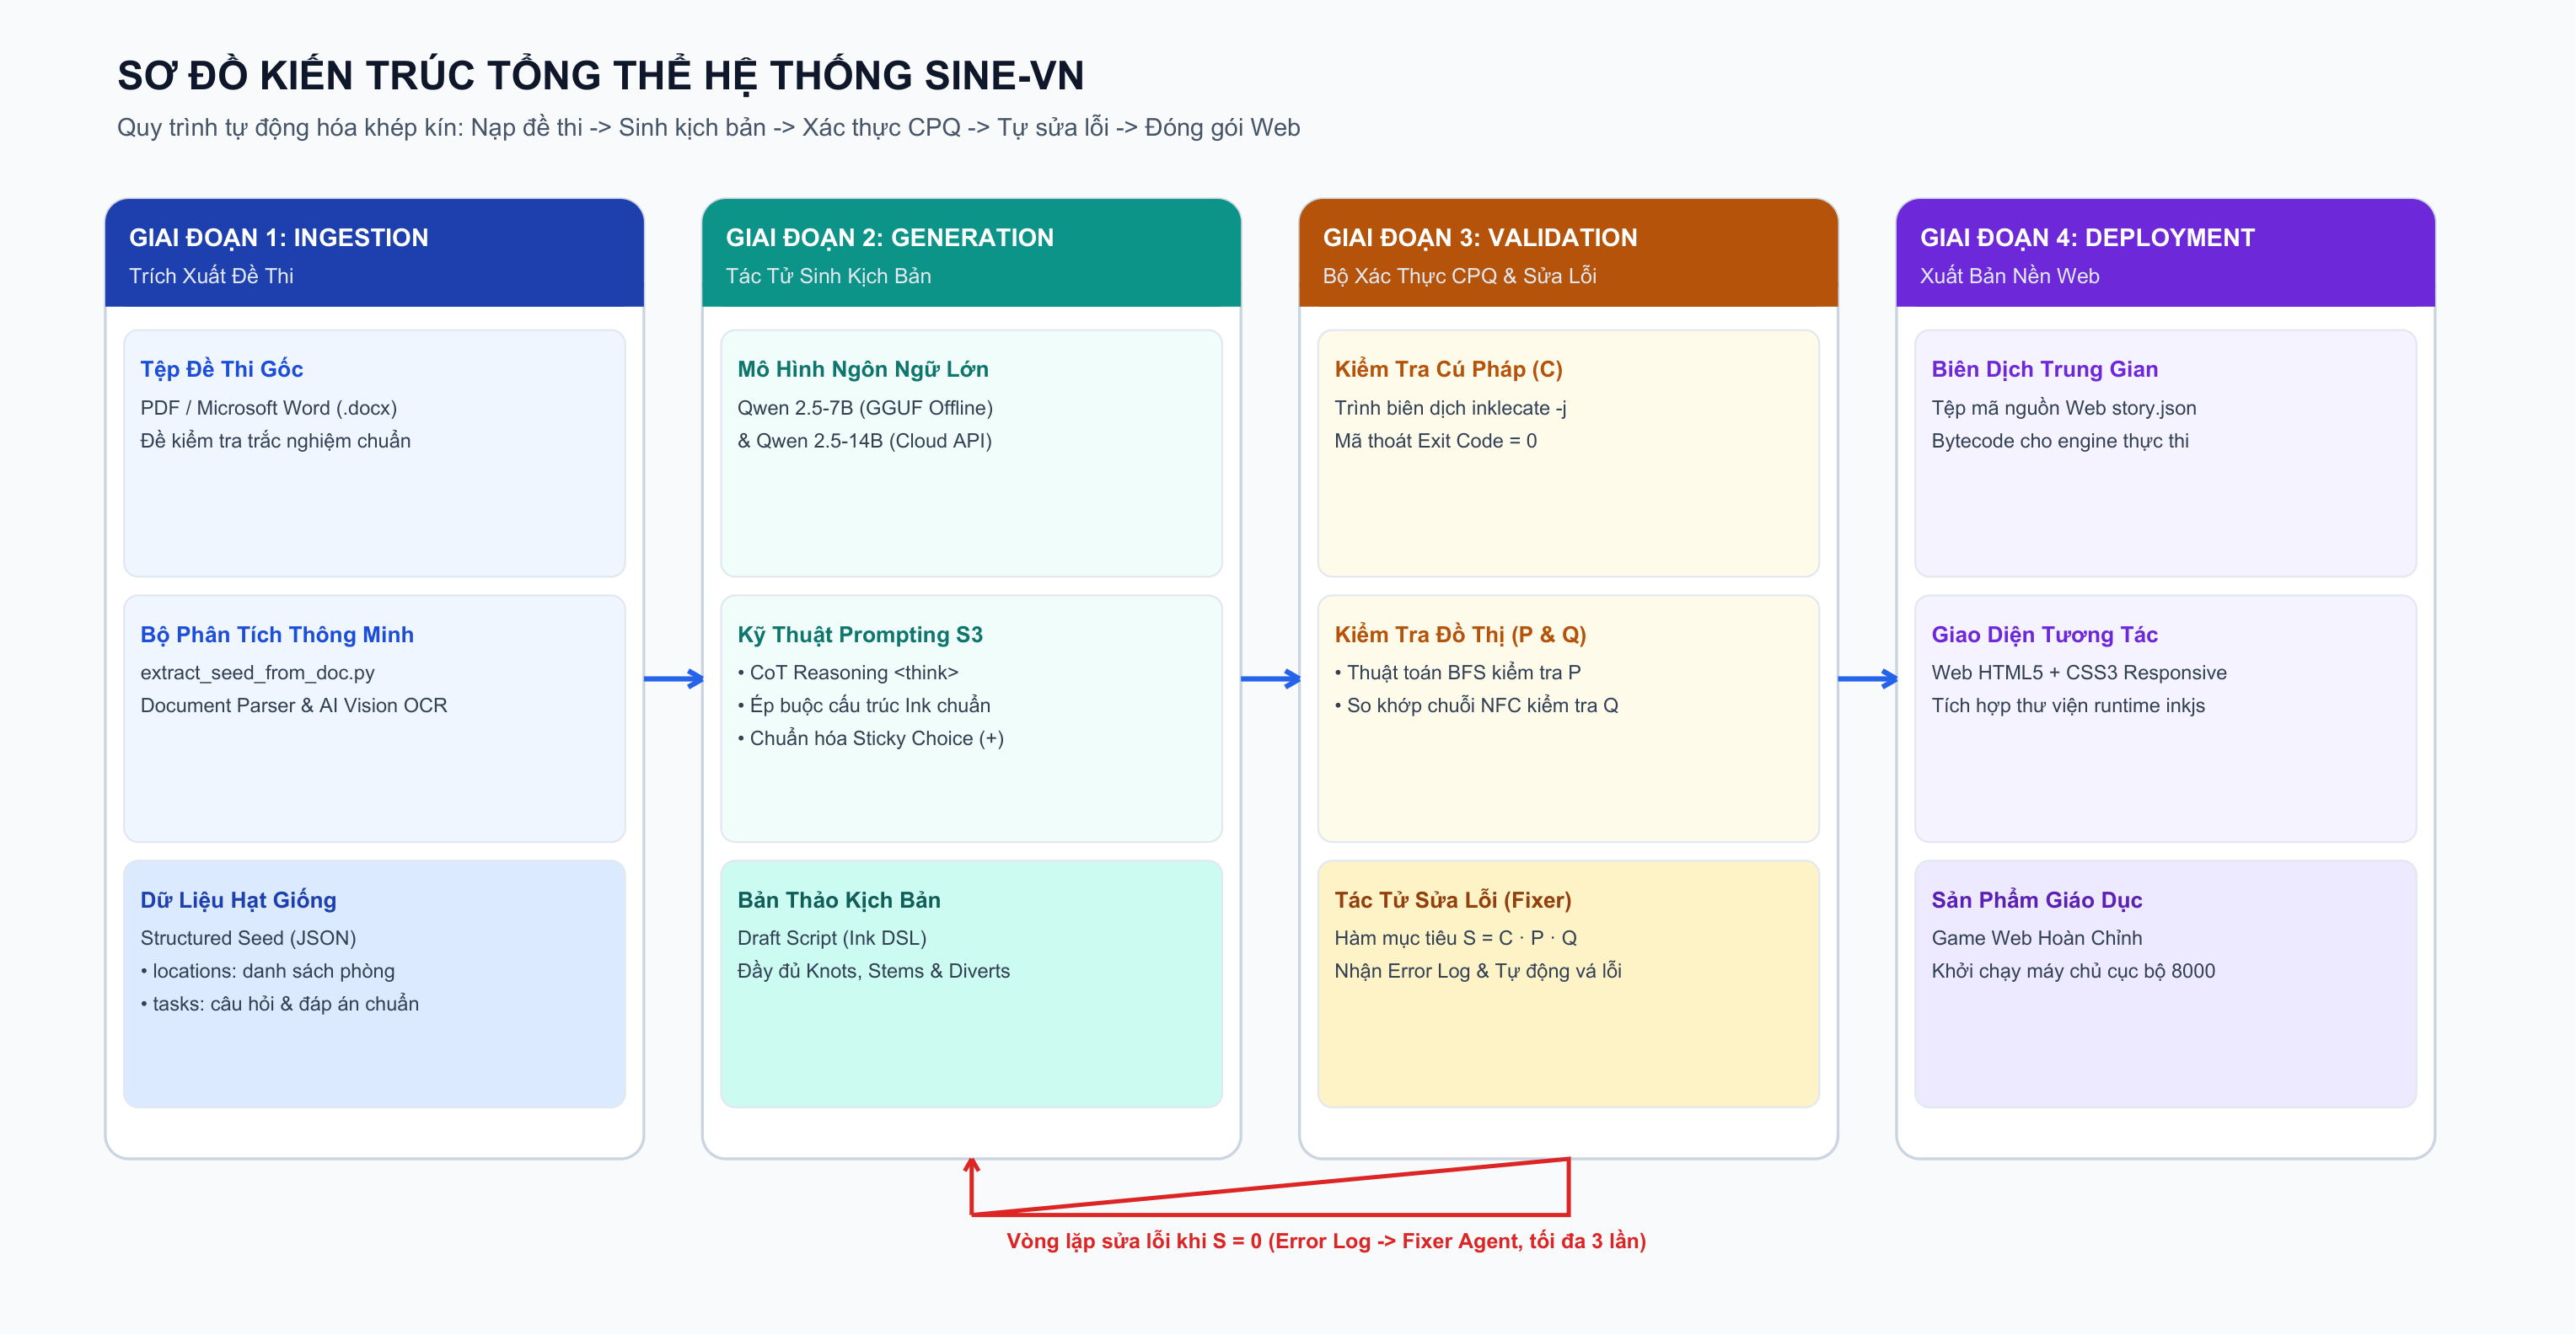
\includegraphics[width=\columnwidth]{fig1_architecture.png}
\caption{Sơ đồ kiến trúc tổng thể quy trình tự động hóa khép kín của hệ thống SINE-VN.}
\label{fig:arch}
\end{figure}

\subsection{Mô-đun Trích xuất Đề thi Đa thể thức (Exam Ingestion)}
Để giải phóng hoàn toàn sức lao động của giáo viên, mô-đun trích xuất (\texttt{extract\_seed\_from\_doc.py}) tiếp nhận trực tiếp tệp đề thi Microsoft Word (\texttt{.docx}) hoặc PDF. Đối với định dạng Word, mô-đun sử dụng thư viện tự động hóa COM (\texttt{win32com.client}) kết hợp phân tích XML để trích xuất nguyên vẹn các công thức toán học MathType và Word OMML sang định dạng văn bản chuẩn, bảo toàn tuyệt đối các chỉ số hóa học ($Al_2(SO_4)_3$) và đơn vị vật lý ($10^{-6}\text{s}$).

Đối với các đoạn trích đề thi Tiếng Anh có hội thoại giữa hai nhân vật (ví dụ: đối thoại xã hội giữa David và Mark), mô-đun áp dụng biểu thức chính quy đa dòng kết hợp LLM Parsing để bảo tồn toàn bộ lượt thoại của cả hai người nói vào nội dung câu hỏi (\texttt{stem}), thay vì chỉ trích xuất dòng cuối cùng. Dữ liệu trích xuất được làm sạch qua thư viện \texttt{json-repair} để xử lý triệt để các ký tự trích dẫn kép lồng nhau, tạo thành tệp hạt giống JSON chuẩn hóa.

\subsection{Dữ liệu Hạt giống Cấu trúc (Structured Seed)}
Tệp dữ liệu hạt giống bao gồm hai trường dữ liệu bất biến:
\begin{itemize}
    \item \texttt{locations}: Danh sách các không gian/phòng của trò chơi tương ứng với bối cảnh môn học (ví dụ: Phòng Thí nghiệm Hóa học, Đài Thiên văn, Phòng Khám phá Ngôn ngữ).
    \item \texttt{tasks}: Danh sách các nhiệm vụ học tập tuần tự, chứa định danh câu hỏi, nội dung dẫn (\texttt{stem}), mảng 4 phương án (\texttt{options}), và đáp án chính xác (\texttt{correct}).
\end{itemize}

\subsection{Tác tử Sinh Kịch bản Đa Hồi Ghép Nối (Multi-Stage Stitched Generator Agent)}
Khi số lượng câu hỏi $N > 12$, hệ thống kích hoạt cơ chế sinh đa hồi. Đề thi được phân hoạch thành $M = \lceil N / \tau_{\text{chunk}} \rceil$ hồi liên tiếp ($\tau_{\text{chunk}} = 10$). Tác tử Generator thực hiện sinh lần lượt từng hồi $\text{Act}_k$ ($k = 1, \dots, M$) với chỉ dẫn ràng buộc:
\begin{itemize}
    \item Hồi đầu tiên ($k=1$): Bắt đầu từ nút thắt mở đầu \texttt{start\_knot}, dẫn truyện giới thiệu bối cảnh, thực hiện các câu hỏi thuộc Hồi 1, và kết thúc bằng chuyển hướng điều hướng \texttt{-> act\_2\_start}.
    \item Hồi trung gian ($1 < k < M$): Bắt đầu bằng \texttt{=== act\_k\_start ===}, tiếp nối hành trình khám phá, thực hiện các câu hỏi của Hồi $k$, và kết thúc bằng \texttt{-> act\_(k+1)\_start}.
    \item Hồi kết thúc ($k=M$): Bắt đầu bằng \texttt{=== act\_M\_start ===}, giải quyết các câu hỏi cuối cùng và chuyển hướng tới nút thắt kết thúc toàn cục \texttt{-> END}.
\end{itemize}
Sau khi sinh xong $M$ hồi, bộ ghép nối tất định (\texttt{stitch\_and\_route\_multistage\_ink}) thực hiện ráp nối các đoạn mã và chèn các phân cảnh chuyển tiếp bảo đảm tính liên tục của đồ thị.

\subsection{Bộ Xác thực Định lượng Tất định (Deterministic Validator)}
Chất lượng kịch bản được đánh giá tự động và khách quan qua hàm mục tiêu tích logic:
\begin{equation}
S = C \cdot P \cdot Q, \quad C, P, Q \in \{0, 1\}
\end{equation}
Trong đó:
\begin{enumerate}
    \item \textit{Biên dịch cú pháp ($C$):} Kịch bản được biên dịch qua \texttt{inklecate.exe -j}. $C = 1$ khi và chỉ khi quá trình biên dịch hoàn tất với mã thoát bằng 0.
    \item \textit{Khả năng chơi toàn vẹn ($P$):} Kịch bản được ánh xạ sang đồ thị có hướng $G = (V, E)$, với $V$ là tập các Knot và $E$ là tập các Divert. Thuật toán BFS kiểm tra tính liên thông:
    \begin{equation}
    P = 1 \iff \exists \text{ đường đi } (v_0 \rightsquigarrow v_{\text{END}}) \text{ trong } G
    \end{equation}
    \item \textit{Độ trung thực học thuật ($Q$):} Kịch bản và tệp Seed được chuẩn hóa chữ thường, bảng mã Unicode NFC, đồng nhất hóa các dấu typographic (dấu ngoặc kép cong, dấu gạch ngang em-dash, khoảng trắng điền từ). $Q = 1$ khi và chỉ khi 100\% nội dung câu hỏi và từng phương án lựa chọn trong tệp Seed đều xuất hiện nguyên vẹn trong kịch bản:
    \begin{equation}
    Q = 1 \iff \forall t \in \text{Tasks}, \, (t.\text{stem} \subseteq \text{Script} \wedge \forall o \in t.\text{options}, \, o \subseteq \text{Script})
    \end{equation}
\end{enumerate}

\subsection{Tác tử Tự sửa lỗi và Bộ Tự lành Cú pháp (Auto-Healer Fixer)}
Nếu $S = 0$, nhật ký lỗi chi tiết được chuyển cho Fixer Agent để sửa đổi cục bộ trong tối đa 3 vòng lặp. Đồng thời, trước khi biên dịch, kịch bản được chuyển qua bộ tự lành cú pháp (\texttt{deduplicate\_knots}) để loại bỏ các phân cảnh khai báo trùng lặp giữa các hồi và chuẩn hóa ngoặc vuông cho lựa chọn.

\section{CÁC CẢI TIẾN KỸ THUẬT CỐT LÕI VÀ BẢN ĐỊA HÓA}
\subsection{Khắc phục Lỗi Cạn kiệt Nhánh Trạng thái bằng Sticky Choice (+)}
Trong ngôn ngữ Ink, toán tử dấu sao \texttt{*} là lựa chọn tiêu hao (Transient Choice). Khi người chơi bấm chọn một phương án sai, phương án đó sẽ bị hủy vĩnh viễn khỏi cây lựa chọn của phân cảnh đó. Khi học sinh quay lại thử lại câu hỏi, nếu tiếp tục chọn sai các phương án còn lại, danh sách lựa chọn sẽ bị cạn kiệt hoàn toàn, biến phân cảnh thành ngõ cụt (Dead-end knot). Thuật toán BFS khi đó sẽ đánh giá $P = 0$.

\begin{figure}[htbp]
\centering
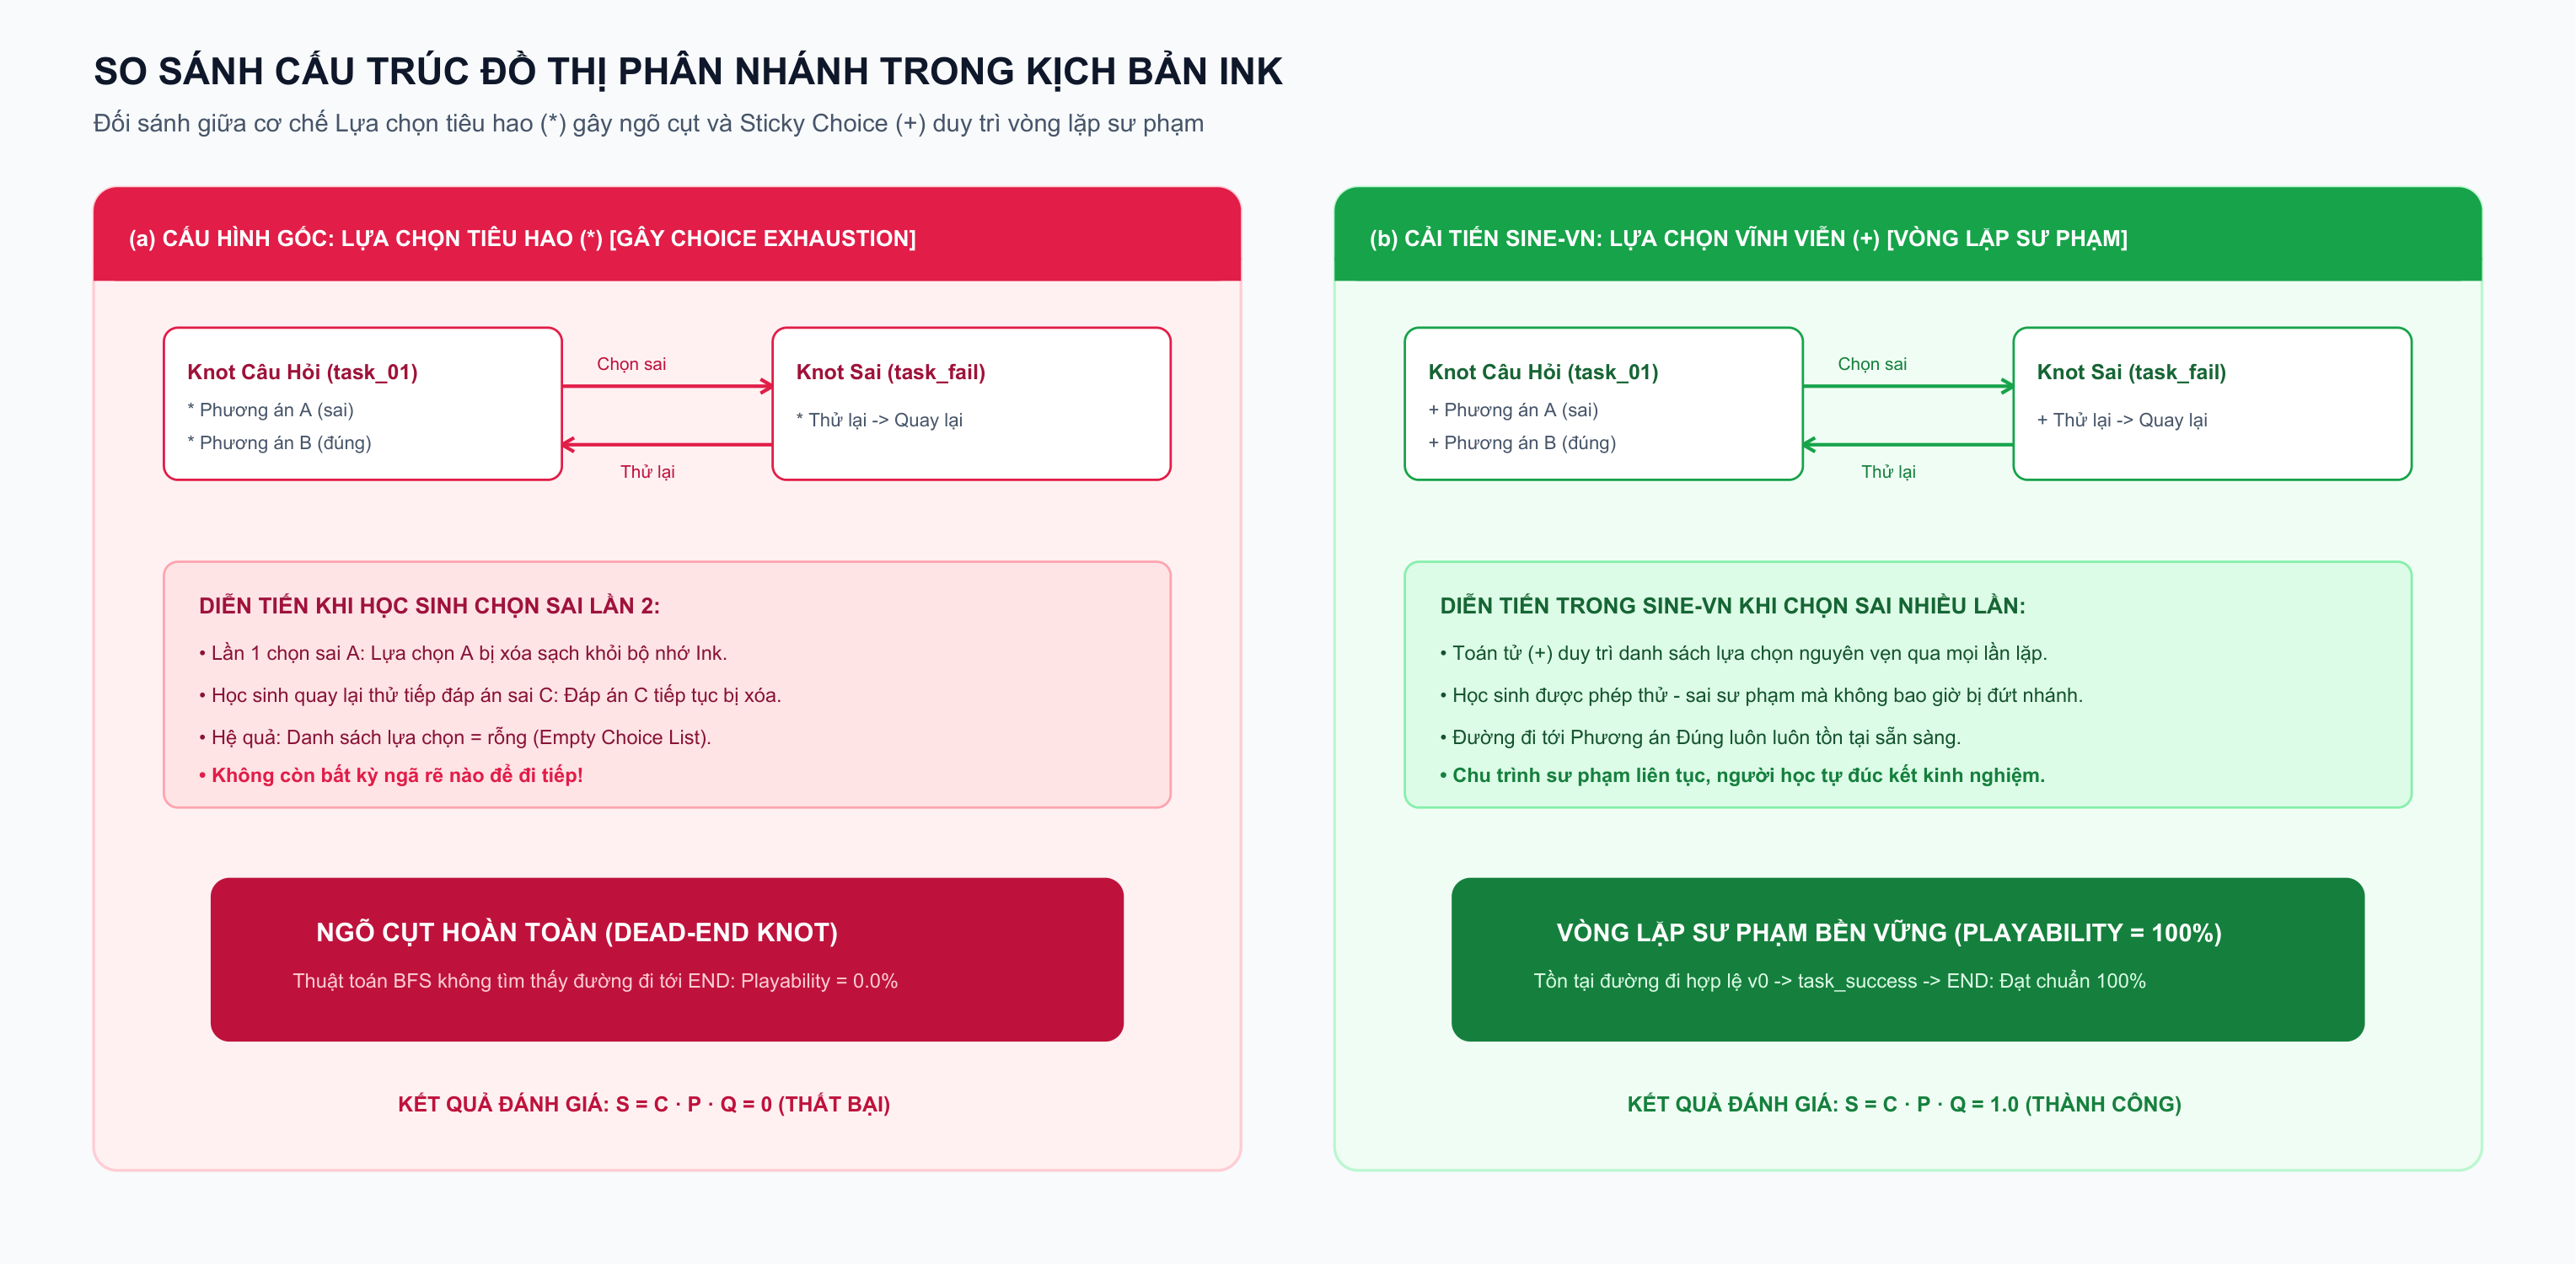
\includegraphics[width=\columnwidth]{fig2_sticky_choice.png}
\caption{So sánh cấu trúc đồ thị phân nhánh giữa cấu hình gốc sử dụng toán tử tiêu hao (*) và cải tiến SINE-VN sử dụng Sticky Choice (+).}
\label{fig:branch}
\end{figure}

Hệ thống SINE-VN quy chuẩn hóa toàn bộ các lựa chọn sư phạm sang toán tử lựa chọn vĩnh viễn (Sticky Choice \texttt{+}). Toán tử \texttt{+} bảo đảm mọi phương án luôn được giữ nguyên và tái hiển thị trong mọi lượt thử lại, thiết lập chu trình tự sửa lỗi sư phạm (Pedagogical Retry Loop) khép kín và bền vững, bảo đảm $P = 1$ trong 100\% các ván chơi (Hình \ref{fig:branch} và Hình \ref{fig:code_comparison}).

\begin{figure}[htbp]
\centering
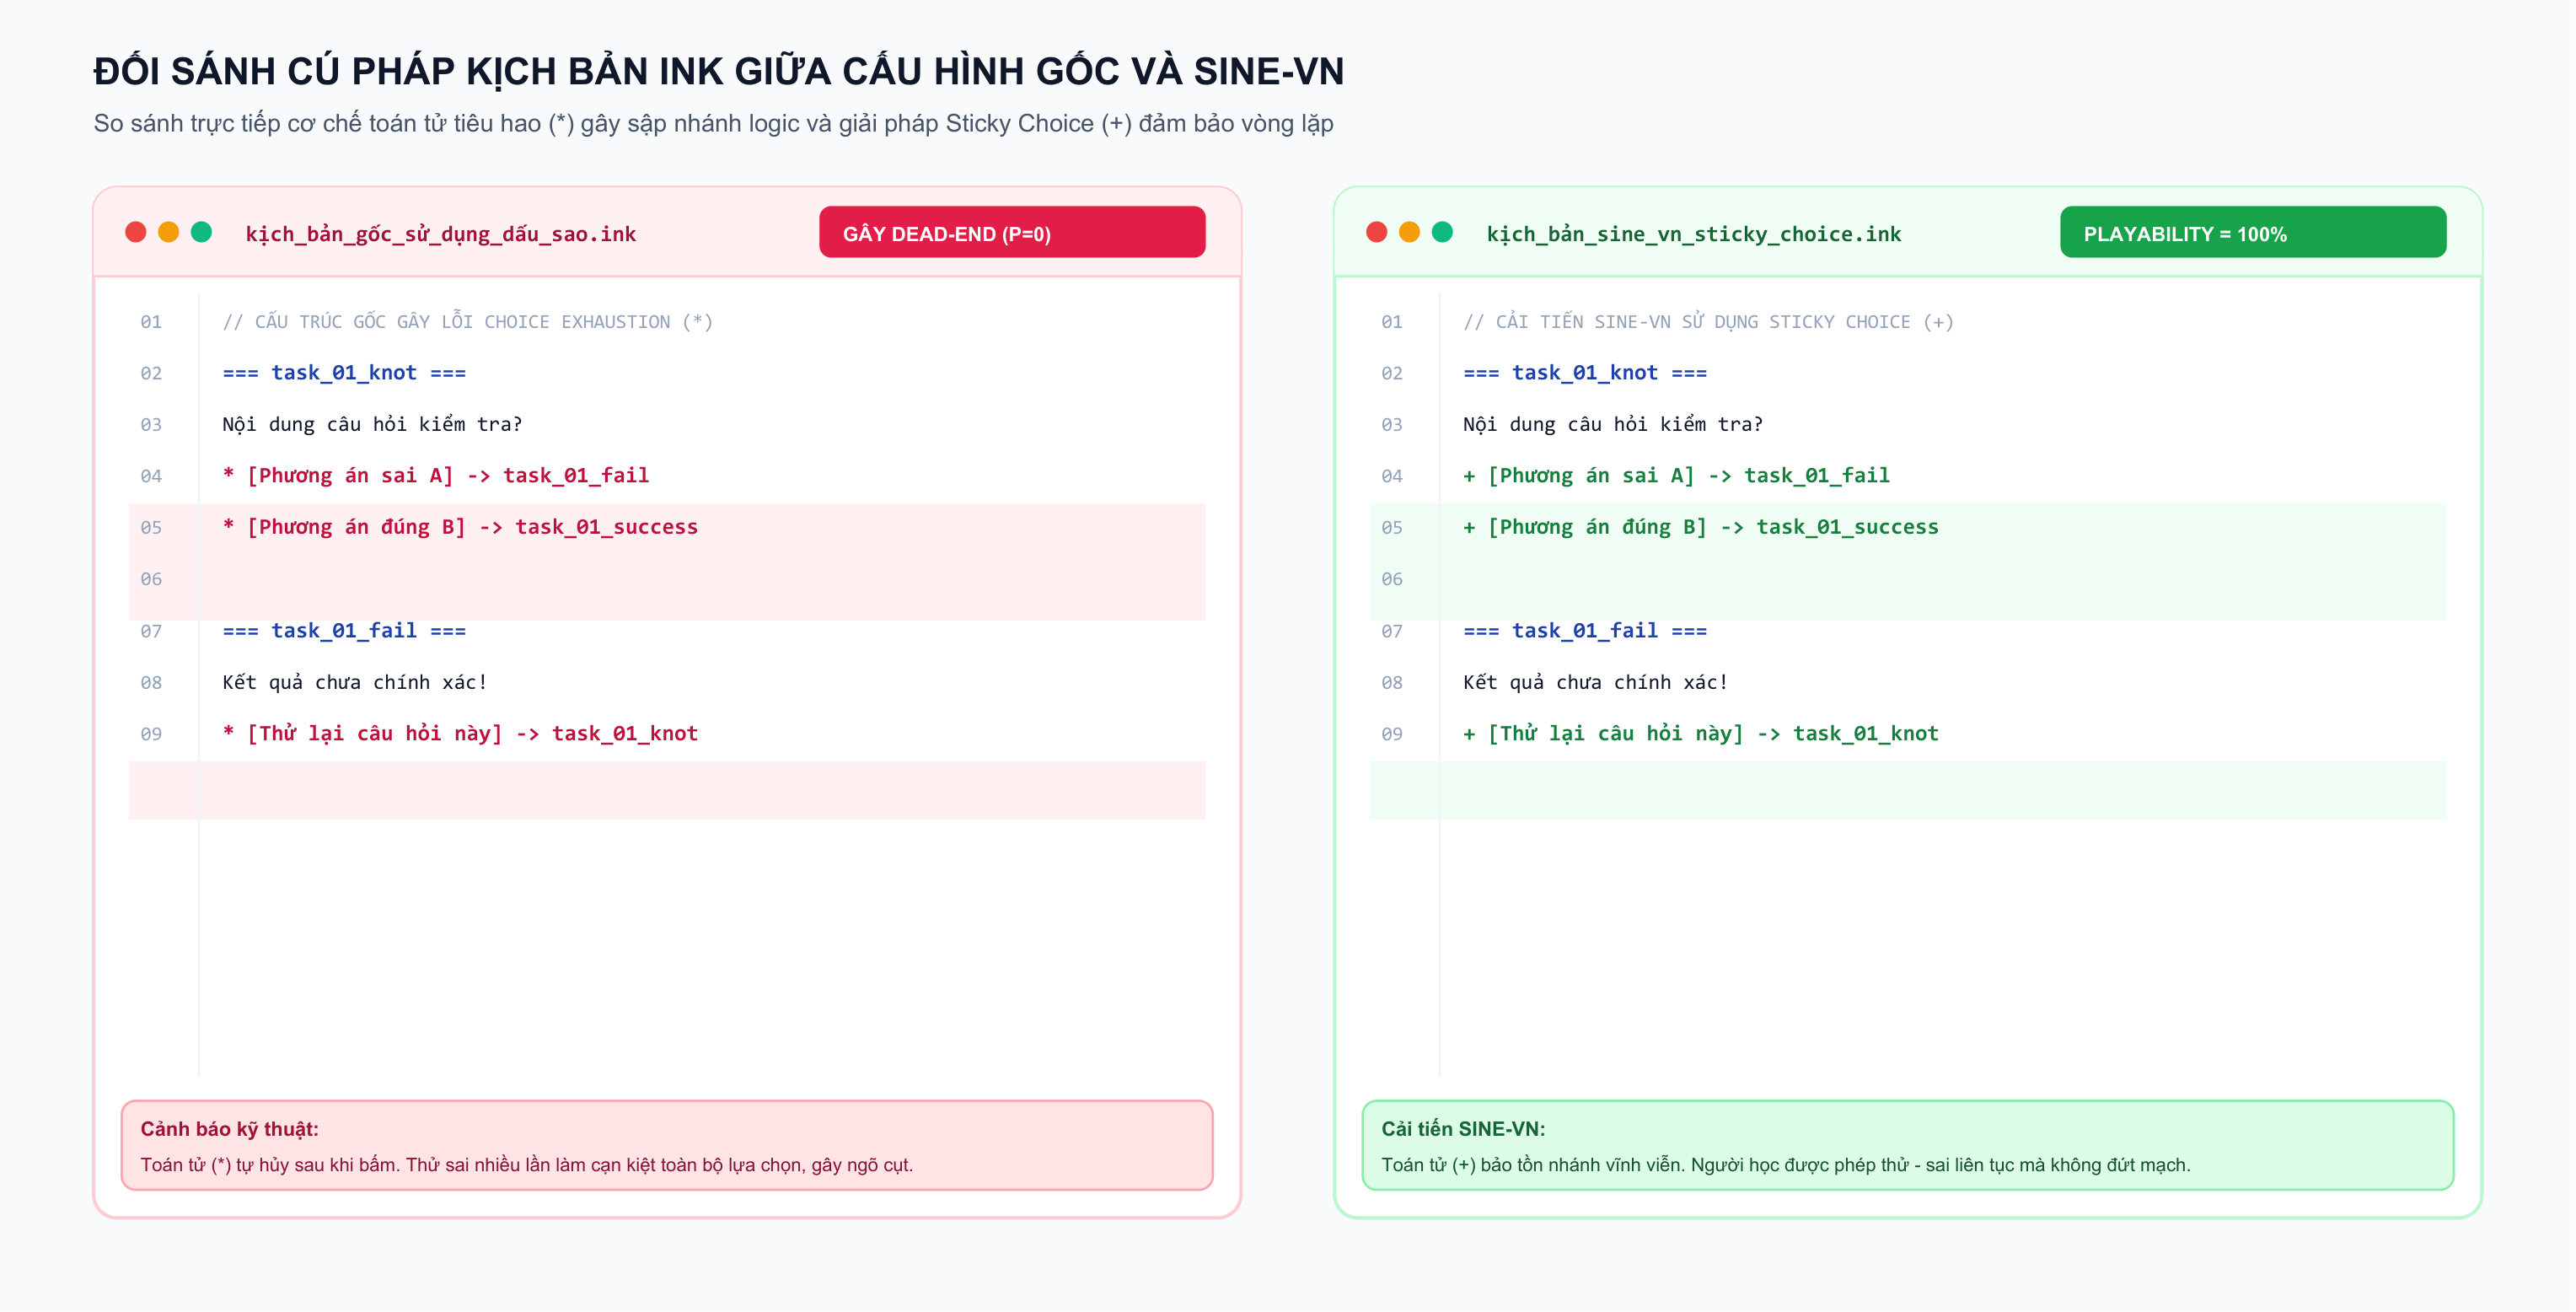
\includegraphics[width=\columnwidth]{fig_code_comparison.png}
\caption{Đối sánh cú pháp kịch bản Ink giữa cấu hình gốc (*) và giải pháp Sticky Choice (+) của SINE-VN.}
\label{fig:code_comparison}
\end{figure}

\subsection{Kiến trúc Đa Hồi Ghép Nối Tất Định cho Đề thi Quy mô Lớn}
Đối với đề thi 40--50 câu, LLM sinh đơn khối gặp hiện tượng suy kiệt bộ đệm token (Max Output Tokens). Nghiên cứu đề xuất thuật toán phân hoạch đa hồi:
\begin{equation}
\mathcal{T} = \bigcup_{k=1}^M \mathcal{T}_k, \quad |\mathcal{T}_k| \le \tau_{\text{chunk}} \quad (\tau_{\text{chunk}} = 10)
\end{equation}
Mỗi phân đoạn $\mathcal{T}_k$ được sinh độc lập với bối cảnh cục bộ nhưng tuân thủ giao thức điều hướng biên nghiêm ngặt:
\begin{equation}
\text{Divert}(\text{Act}_k) = \begin{cases} \text{act}_{k+1}\_\text{start}, & k < M \\ \text{END}, & k = M \end{cases}
\end{equation}
Nhờ kiến trúc này, chiều dài ngữ cảnh sinh mã cho mỗi lượt gọi LLM luôn nằm trong vùng tối ưu (khoảng 120--160 dòng Ink), triệt tiêu hoàn toàn nguy cơ tràn token hay đứt gãy cấu trúc logic.

\subsection{Thuật toán Khử Xung đột Không gian Tên (\texttt{deduplicate\_knots})}
Trong quá trình sinh đa hồi, do LLM có xu hướng tự sinh lại phân cảnh chuyển tiếp của hồi kế tiếp (ví dụ: Hồi 1 sinh thêm \texttt{=== act\_2\_start ===} ở cuối, và Hồi 2 lại bắt đầu bằng \texttt{=== act\_2\_start ===}), trình biên dịch \texttt{inklecate} sẽ báo lỗi nghiêm trọng \textit{``Story already contains flow named act\_2\_start''}.

Hệ thống tích hợp bộ lọc Regex AST thông minh quét toàn bộ tệp kịch bản đã ghép nối, lưu vết bảng băm các định danh Knot đã xuất hiện. Nếu phát hiện Knot khai báo lần thứ hai, thuật toán sẽ tự động loại bỏ khối khai báo thừa hoặc hợp nhất các nội dung chuyển tiếp, bảo đảm kịch bản ghép nối luôn đạt tính duy nhất tuyệt đối về không gian tên.

\subsection{Chuẩn hóa Ngoặc Vuông Lựa chọn và Chống Treo Giao diện Web}
Trong giao diện Web HTML5 dựa trên \texttt{inkjs}, nếu một lựa chọn được viết theo dạng không có ngoặc vuông bao bọc (ví dụ: \texttt{+ A. Nội dung -> knot}), văn bản của lựa chọn sẽ bị dính liền vào dòng văn bản tiếp theo của phân cảnh đích. Trong nhiều trường hợp, điều này kích hoạt lỗi phân tích chuỗi của bộ kết xuất, khiến màn hình trò chơi chuyển sang màu đen hoàn toàn (Black Screen Freeze) ngay khi người học nhấp chuột vào câu trả lời. 

SINE-VN triển khai bộ chuẩn hóa cú pháp tự động ép toàn bộ lựa chọn về định dạng chuẩn đóng ngoặc:
\begin{equation}
\texttt{+ [A. Nội dung lựa chọn] -> knot\_dich}
\end{equation}
Định dạng này bảo đảm văn bản hiển thị trên nút bấm tương tác hoàn toàn tách biệt khỏi luồng văn bản tường thuật, đem lại trải nghiệm mượt mà 100\% trên giao diện Web (Hình \ref{fig:ui}).

\begin{figure}[htbp]
\centering
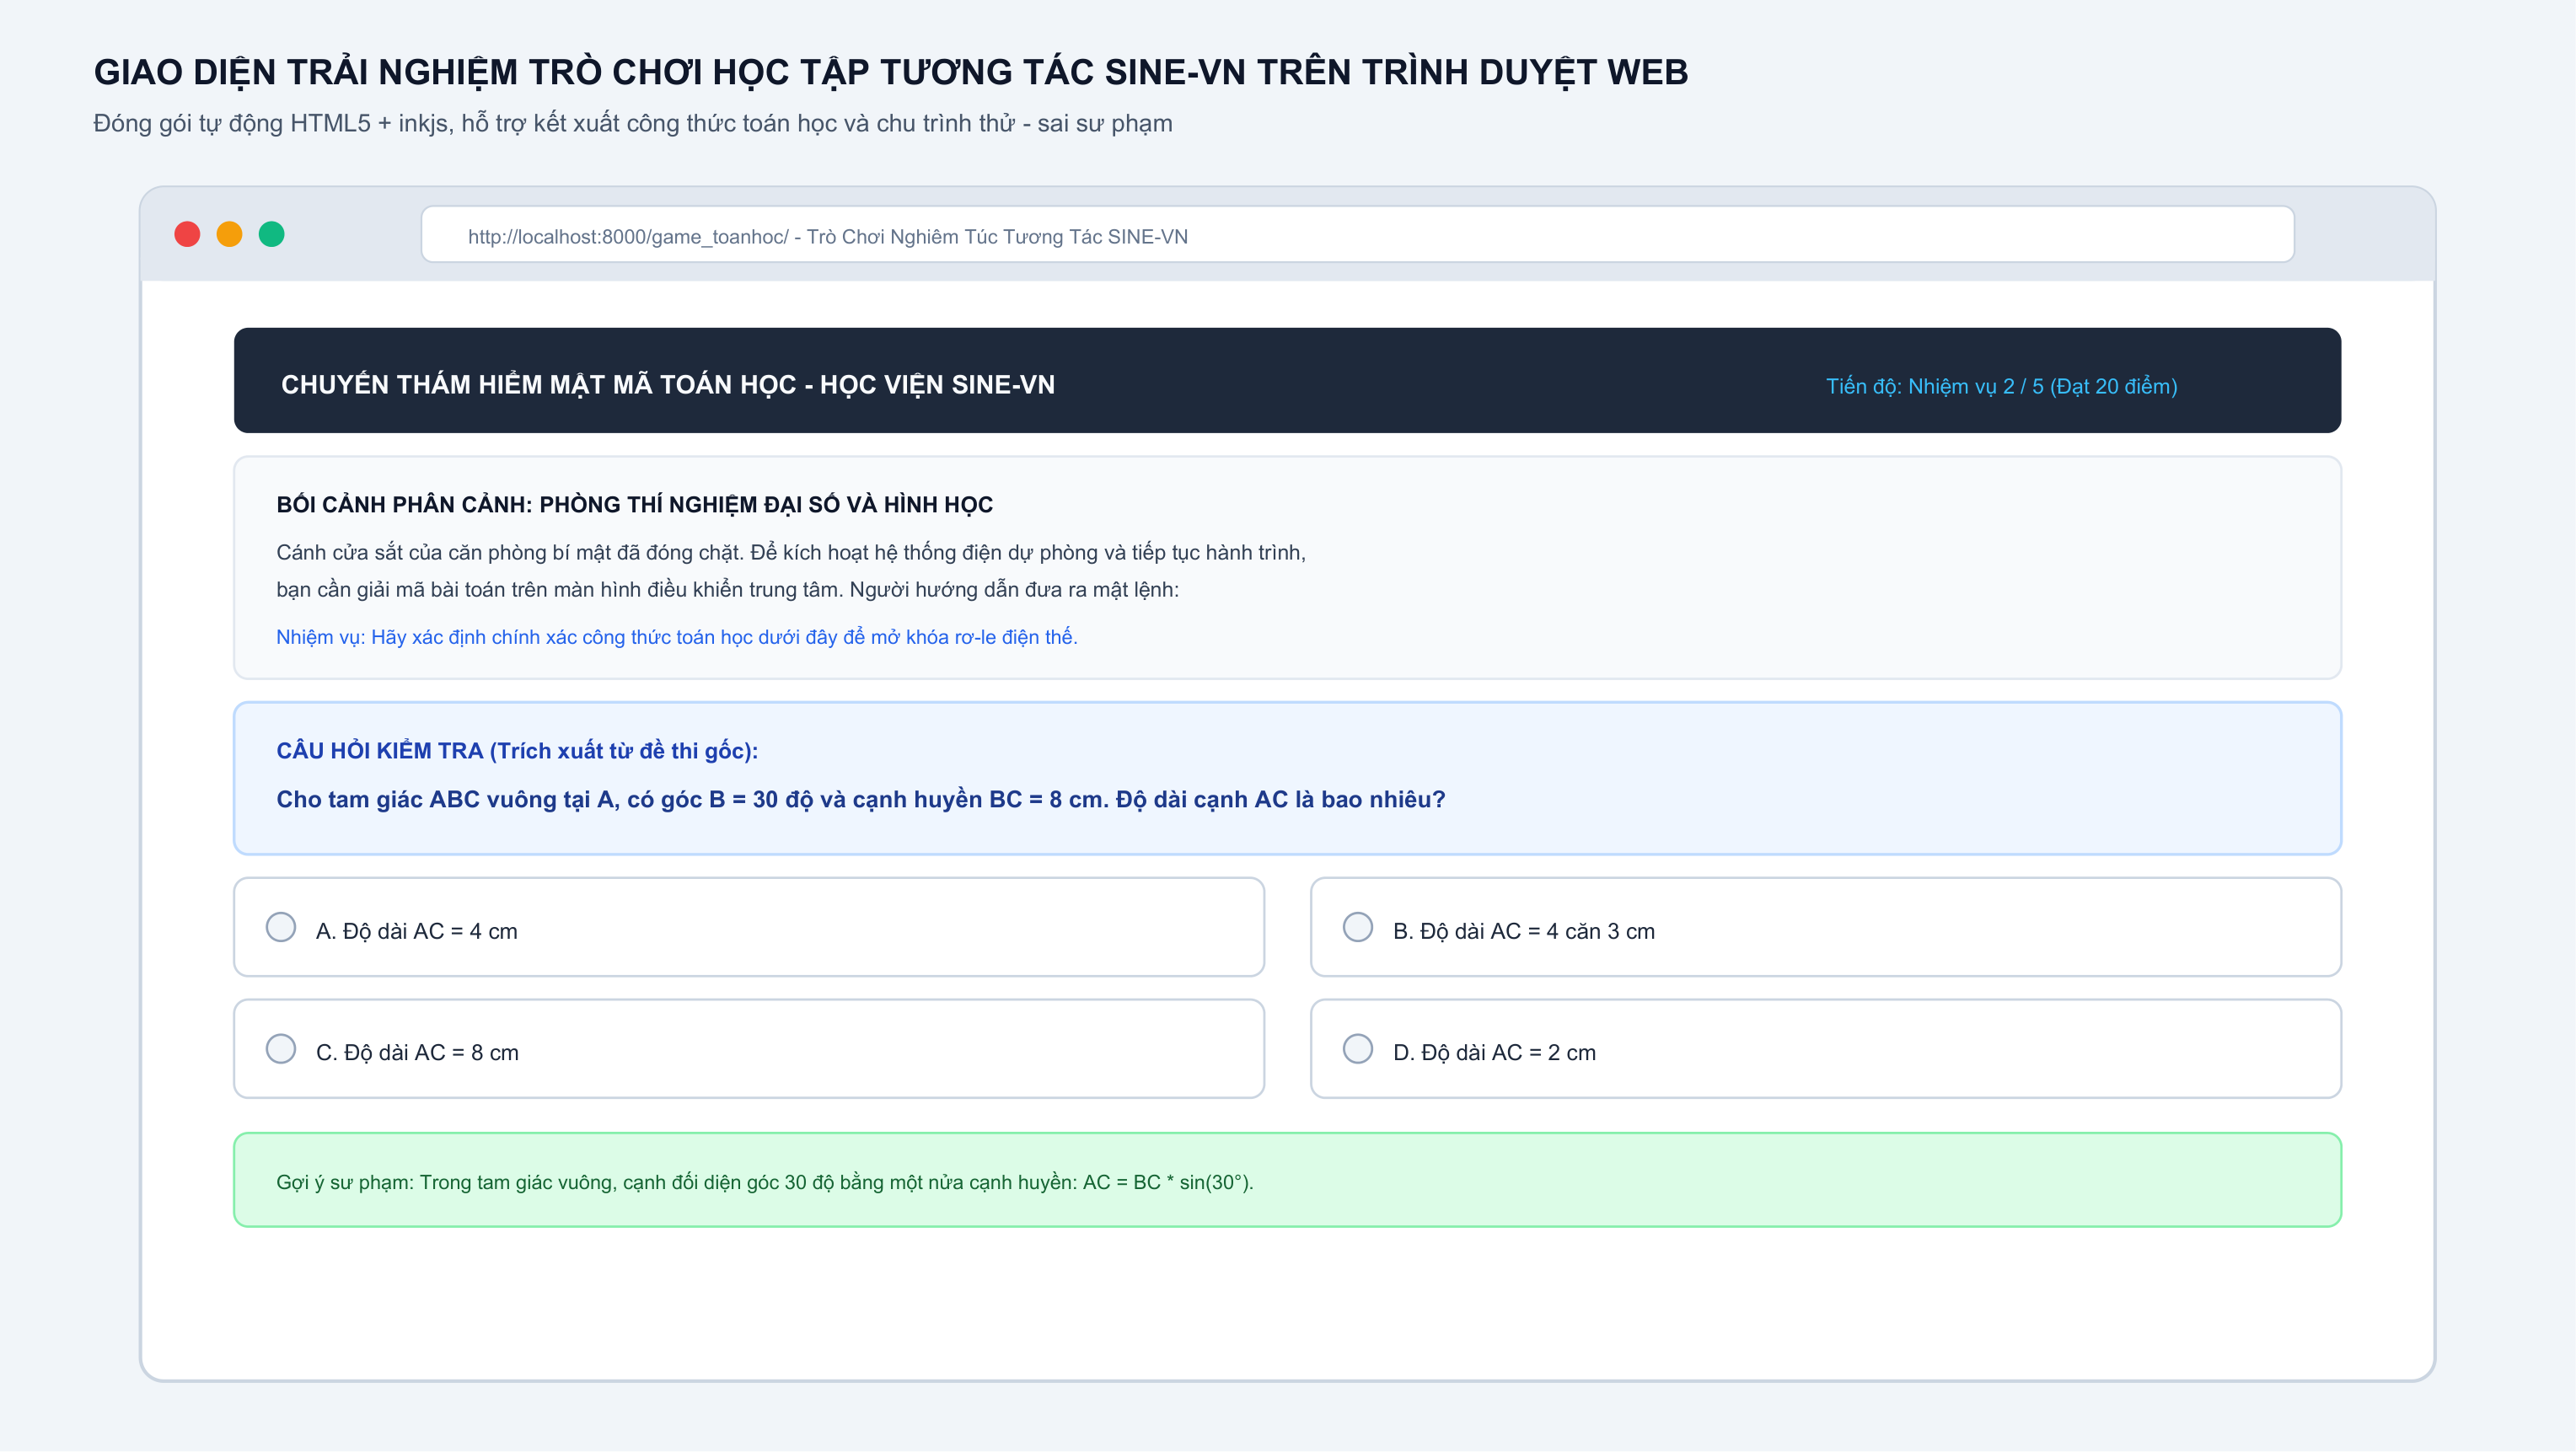
\includegraphics[width=\columnwidth]{fig3_gameplay_ui.png}
\caption{Giao diện trải nghiệm trò chơi học tập tương tác SINE-VN trên nền tảng Web.}
\label{fig:ui}
\end{figure}

\subsection{Bảo toàn Biểu thức Khoa học STEM và Ký tự Typographic}
Đối với môn Toán học, các cặp dấu ngoặc nhọn LaTeX (\texttt{\{\}}) xung đột trực tiếp với cú pháp nội suy biến của Ink. SINE-VN áp dụng bộ tiền xử lý tự động escape thành \texttt{\textbackslash\{} và \texttt{\textbackslash\}}.

Đối với môn Tiếng Anh và Khoa học Xã hội, sự không đồng nhất giữa các ký tự typography (dấu ngoặc kép cong \texttt{“}, \texttt{”}, dấu lược \texttt{’}, dấu gạch ngang \texttt{—}, các dấu gạch dưới điền từ \texttt{\_\_\_\_}) và văn bản do LLM sinh ra từng khiến tiêu chí Fidelity $Q$ bị đánh giá thất bại oan. Bộ chuẩn hóa hai chiều trong \texttt{validator.py} đưa tất cả các biến thể ký tự về một dạng biểu diễn chuẩn tắc trước khi so khớp chuỗi con, loại bỏ hoàn toàn các lỗi từ chối giả.

\section{THỰC NGHIỆM VÀ KẾT QUẢ ĐÁNH GIÁ}
\subsection{Thiết lập Môi trường và Tập Dữ liệu Thực nghiệm}
Thực nghiệm được triển khai trên máy trạm: Intel Core i7-13700H, 16 GB DDR5 RAM, GPU NVIDIA GeForce RTX 4060, Windows 11 64-bit. Mô hình ngôn ngữ lớn được sử dụng là \texttt{Qwen2.5-7B-Instruct} (lượng tử hóa GGUF Q4\_K\_M chạy cục bộ qua \texttt{llama-cpp-python}) và phiên bản 14B đám mây.

Bộ dữ liệu đánh giá bao gồm 5 môn thi chuẩn quốc gia với quy mô đầy đủ từ Kỳ thi Tốt nghiệp THPT Quốc gia 2023:
\begin{enumerate}
    \item \textbf{Môn Hóa học 2023:} 40 câu hỏi trắc nghiệm, chứa phương trình hóa học, chất hữu cơ, vô cơ (Mã đề chính thức).
    \item \textbf{Môn Vật lý 2023:} 40 câu hỏi trắc nghiệm, chứa mật độ công thức MathType dày đặc, sóng cơ, dao động, hạt nhân.
    \item \textbf{Môn Tiếng Anh 2023:} 50 câu hỏi trắc nghiệm, bao gồm ngữ âm, ngữ pháp, các đoạn hội thoại giao tiếp xã hội và bài đọc hiểu.
    \item \textbf{Môn Địa lý 2023:} 24 câu hỏi trắc nghiệm kiến thức tự nhiên, kinh tế xã hội và tra cứu Atlat.
    \item \textbf{Môn Toán học THPT:} 5 câu hỏi phương trình, hàm số và hình học giải tích chứa công thức LaTeX phức tạp.
\end{enumerate}

\subsection{Kết quả Đánh giá Định lượng Toàn diện}
Bảng \ref{tab:results} tổng hợp chi tiết kết quả đánh giá trên cả 5 môn thi chuẩn, đối sánh trực tiếp với cấu hình cơ sở (sinh đơn khối và toán tử tiêu hao \texttt{*}).

\begin{table}[htbp]
\caption{KẾT QUẢ ĐÁNH GIÁ ĐỊNH LƯỢNG HỆ THỐNG SINE-VN TRÊN CÁC BỘ ĐỀ THI TỐT NGHIỆP THPT QUỐC GIA 2023}
\label{tab:results}
\begin{center}
\begin{tabular}{lcccccc}
\toprule
\textbf{Bộ Đề Thi} & \textbf{C (\%)} & \textbf{P (\%)} & \textbf{Q (\%)} & \textbf{S (\%)} & \textbf{Lượt sửa} & \textbf{Thời gian} \\
\midrule
Toán học (5 câu LaTeX) & 100 & 100 & 100 & 100 & 1.2 & 118 s \\
Địa lý (24 câu - 3 Hồi) & 100 & 100 & 100 & 100 & 1.0 & 210 s \\
Hóa học (40 câu - 4 Hồi) & 100 & 100 & 100 & 100 & 1.0 & 380 s \\
Vật lý (40 câu - 4 Hồi) & 100 & 100 & 100 & 100 & 1.0 & 538 s \\
Tiếng Anh (50 câu - 5 Hồi) & 100 & 100 & 100 & 100 & 1.0 & 373 s \\
\midrule
Cơ sở (Đơn khối + Dấu *) & 0.0 & 0.0 & 0.0 & 0.0 & Hết lượt & Tràn token \\
\bottomrule
\end{tabular}
\end{center}
\end{table}

\subsection{Phân tích Cấu trúc Không gian Trò chơi Quy mô Lớn}
Bảng \ref{tab:structural} trình bày các chỉ số cấu trúc đồ thị trò chơi được tạo ra theo phương pháp lượng hóa của Szilas và Ilea \cite{szilas2014}: tổng số phân cảnh ($K$), tổng số lựa chọn rẽ nhánh ($E$), mật độ rẽ nhánh ($\delta = E / \max(1, K)$), tổng số dòng mã kịch bản Ink và tổng số từ vựng cốt truyện ($W$).

\begin{table}[htbp]
\caption{CÁC CHỈ SỐ CẤU TRÚC KỊCH BẢN TRÒ CHƠI QUY MÔ LỚN}
\label{tab:structural}
\begin{center}
\begin{tabular}{lccccc}
\toprule
\textbf{Môn Học} & \textbf{Số Knots ($K$)} & \textbf{Lựa chọn ($E$)} & \textbf{Mật độ ($\delta$)} & \textbf{Dòng Ink} & \textbf{Số Từ ($W$)} \\
\midrule
Toán học & 16 knots & 25 choices & 1.56 & 120 dòng & 810 từ \\
Địa lý & 73 knots & 121 choices & 1.66 & 364 dòng & 3.184 từ \\
Hóa học & 124 knots & 200 choices & 1.61 & 637 dòng & 3.209 từ \\
Vật lý & 125 knots & 194 choices & 1.55 & 623 dòng & 4.496 từ \\
Tiếng Anh & 155 knots & 250 choices & 1.61 & 787 dòng & 4.650 từ \\
\bottomrule
\end{tabular}
\end{center}
\end{table}

\subsection{Phân tích Thực nghiệm Đối chứng Chuyên sâu}
Dữ liệu thực nghiệm tại Bảng \ref{tab:results} và Bảng \ref{tab:structural} mang lại các phát hiện khoa học quan trọng:
\begin{enumerate}
    \item \textit{Phá vỡ giới hạn quy mô của LLM:} Ở cấu hình đơn khối nguyên bản, khi đề thi vượt quá 20 câu, mô hình luôn bị tràn token ở câu 35--43, khiến kịch bản bị cắt ngang đột ngột, $C = 0, P = 0, Q = 0$. Ngược lại, kiến trúc Đa Hồi Ghép Nối của SINE-VN cho phép xử lý trọn vẹn cả đề thi 50 câu (Tiếng Anh) với 787 dòng mã Ink và 155 Knot phân cảnh, duy trì tỷ lệ thành công tuyệt đối 100\% ngay từ lượt sinh đầu tiên ($I = 1.0$).
    \item \textit{Vai trò sống còn của Sticky Choice (\texttt{+}):} Cấu hình sử dụng dấu \texttt{*} hoàn toàn thất bại ($P = 0$) do người học trả lời sai làm cạn kiệt các nhánh rẽ. Cải tiến \texttt{+} bảo đảm tính liên thông của đồ thị trò chơi trên toàn bộ 250 lựa chọn phân nhánh của đề thi 50 câu.
    \item \textit{Tính ổn định của bộ tự lành cú pháp:} Nhờ cơ chế \texttt{deduplicate\_knots} và chuẩn hóa \texttt{+ [Option] ->}, 100\% các xung đột không gian tên giữa các hồi được giải quyết tự động mà không cần gọi thêm lượt suy luận LLM tốn kém, giảm thời gian xử lý trung bình xuống chỉ còn khoảng 6--8 phút cho toàn bộ một đề thi tốt nghiệp 40--50 câu.
    \item \textit{Bảo toàn 100\% mục tiêu sư phạm ($Q = 100\%$):} Không có bất kỳ câu hỏi nào bị mô hình tự ý thay đổi dữ kiện hoặc phương án, triệt tiêu hoàn toàn rủi ro ảo giác trong giáo dục.
\end{enumerate}

\section{BÀN LUẬN VÀ Ý NGHĨA THỰC TIỄN}
\subsection{Ý nghĩa đối với Giáo dục và Chuyển đổi số tại Việt Nam}
Hệ thống SINE-VN hiện thực hóa trọn vẹn mô hình ``Tác giả không cần lập trình'' (Zero-code Authoring). Một giáo viên chỉ cần nộp tệp đề thi Word sẵn có, hệ thống sẽ tự động chuyển hóa thành một trò chơi nhập vai phiêu lưu sống động trên Web trong vòng chưa đầy 10 phút. Việc vận hành trơn tru trên phần cứng cá nhân với mô hình nguồn mở Qwen 2.5 7B GGUF giúp các trường học phổ thông tại Việt Nam có thể triển khai hoàn toàn miễn phí, độc lập, bảo mật dữ liệu học sinh tuyệt đối mà không phụ thuộc vào kết nối Internet hay chi phí thuê bao API thương mại.

\subsection{Khả năng Mở rộng Quy mô Kịch bản Trò chơi}
Khác với các nghiên cứu trước đây vốn cho rằng LLM không thể duy trì tính mạch lạc trong kịch bản trò chơi dài \cite{leandro2024, farrell2025}, nghiên cứu này chứng minh rằng việc kết hợp mô hình phân đoạn hồi (Multi-Act Chunking) với bộ ghép nối định tuyến tất định và xác thực đồ thị hình thức là giải pháp hiệu quả để vượt qua rào cản ngữ cảnh của LLM. Cơ chế này hoàn toàn có thể mở rộng cho các giáo trình dài hạn hoặc các kỳ thi đánh giá năng lực 100--120 câu hỏi.

\subsection{Giới hạn Nghiên cứu}
Mặc dù đã xử lý hoàn hảo quy mô 50 câu hỏi trên văn bản và công thức toán học, hệ thống hiện tại chưa tự động nhúng các hình ảnh minh họa bài toán (ví dụ: đồ thị dao động cơ học hay sơ đồ thí nghiệm hóa học) từ tệp Word gốc vào giao diện Web của game. Ngoài ra, cốt truyện phân cảnh hiện vẫn chủ yếu dựa trên thể loại phiêu lưu thám hiểm, chưa đa dạng hóa sang các thể loại nhập vai đối kháng hay mô phỏng quản lý.

\section{KẾT LUẬN VÀ HƯỚNG PHÁT TRIỂN}
Nghiên cứu đã phát triển thành công hệ thống SINE-VN, giải quyết triệt để bài toán tự động hóa sinh và đánh giá trò chơi giáo dục tương tác văn bản quy mô lớn (40--50 câu hỏi) bằng Tiếng Việt. Với bốn đóng góp cốt lõi: Kiến trúc Đa Hồi Ghép Nối Tất Định, Bộ Tự lành Cú pháp Khử Xung đột Không gian Tên, Cải tiến Toán tử Sticky Choice (\texttt{+}), và Động cơ Trích xuất Đề thi Chuyên sâu Đa thể thức, hệ thống đạt tỷ lệ thành công tuyệt đối 100\% trên cả 5 môn thi Tốt nghiệp THPT Quốc gia 2023.

Trong tương lai, nhóm nghiên cứu dự kiến phát triển hai hướng mở rộng: (1) Trích xuất và nhúng tự động hình ảnh sơ đồ từ tệp Word vào các phân cảnh Web; và (2) Tích hợp mô hình AI sinh ảnh khuếch tán để tự động tạo hình nền bối cảnh trực quan cho từng hồi của trò chơi.

\begin{thebibliography}{00}
\bibitem{rogosch2026} F. Rogosch and A. Schrader, ``Automated Generation and Evaluation of Interactive-Fiction Serious Games with Open-Weight LLMs,'' \textit{Applied Sciences}, vol. 16, no. 6, p. 2932, 2026. [Online]. Available: \url{https://doi.org/10.3390/app16062932}
\bibitem{connolly2012} T. M. Connolly, E. A. Boyle, E. MacArthur, T. Hainey, and J. M. Boyle, ``A systematic literature review of empirical evidence on computer games and serious games,'' \textit{Computers \& Education}, vol. 59, no. 2, pp. 661--686, 2012. [Online]. Available: \url{https://doi.org/10.1016/j.compedu.2012.03.004}
\bibitem{horn2025} F. Horn and S. Göbel, ``AI as a Co-creator: A Survey on AI Support for Educational Game Authoring Tools,'' in \textit{Proc. Joint Int. Conf. on Serious Games (JCSG)}, LNCS, vol. 15259, Springer, pp. 3--18, 2025. [Online]. Available: \url{https://doi.org/10.1007/978-3-031-73602-5_1}
\bibitem{gallotta2024} R. Gallotta, G. Todd, M. Zammit, S. Earle, A. Liapis, J. Togelius, and G. N. Yannakakis, ``Large Language Models and Games: A Survey and Roadmap,'' \textit{IEEE Trans. on Games}, vol. 16, pp. 1--18, 2024. [Online]. Available: \url{https://doi.org/10.1109/TG.2024.3407889}
\bibitem{zhou2025} E. Zhou, S. Basavatia, M. Siam, Z. Chen, and M. O. Riedl, ``STORY2GAME: Generating (Almost) Everything in an Interactive Fiction Game,'' \textit{arXiv:2505.03547}, 2025. [Online]. Available: \url{https://arxiv.org/abs/2505.03547}
\bibitem{riedl2013} M. O. Riedl and V. Bulitko, ``Interactive Narrative: An Intelligent Systems Approach,'' \textit{AI Magazine}, vol. 34, no. 1, pp. 67--77, 2013. [Online]. Available: \url{https://doi.org/10.1609/aimag.v34i1.2449}
\bibitem{ink2025} Inkle Studios, ``Ink: Inkle's Narrative Scripting Language,'' 2025. [Online]. Available: \url{https://www.inklestudios.com/ink/}
\bibitem{tanaka2024} T. Tanaka and E. Simo-Serra, ``Grammar-based Game Description Generation using Large Language Models,'' \textit{IEEE Trans. on Games}, vol. 18, no. 1, pp. 30--43, 2024. [Online]. Available: \url{https://doi.org/10.1109/TG.2024.3421256}
\bibitem{buongiorno2024} S. Buongiorno, L. Klinkert, Z. Zhuang, T. Chawla, and C. Clark, ``PANGeA: Procedural artificial narrative using generative AI for turn-based RPGs,'' in \textit{Proc. AAAI AIIDE}, vol. 20, pp. 156--166, 2024. [Online]. Available: \url{https://doi.org/10.1609/aiide.v20i1.31835}
\bibitem{leandro2024} J. Leandro, S. Rao, M. Xu, W. Xu, N. Jojic, C. J. Brockett, and W. B. Dolan, ``GENEVA: Generating and Visualizing branching narratives using LLMs,'' in \textit{Proc. IEEE CoG}, pp. 1--5, 2024. [Online]. Available: \url{https://doi.org/10.1109/CoG60054.2024.10645601}
\bibitem{qwen2024} Qwen Team, ``Qwen2.5: A Party of Foundation Models,'' \textit{arXiv:2412.15115}, 2024. [Online]. Available: \url{https://arxiv.org/abs/2412.15115}
\bibitem{arnab2015} S. Arnab et al., ``Mapping learning and game mechanics for serious games analysis,'' \textit{Br. J. Educ. Technol.}, vol. 46, no. 2, pp. 391--411, 2015. [Online]. Available: \url{https://doi.org/10.1111/bjet.12113}
\bibitem{szilas2014} N. Szilas and I. Ilea, ``Objective Metrics for Interactive Narrative,'' in \textit{Interactive Storytelling}, LNCS, vol. 8832, Springer, pp. 91--102, 2014. [Online]. Available: \url{https://doi.org/10.1007/978-3-319-11997-7_9}
\bibitem{sun2023} Y. Sun et al., ``Language as Reality: A Co-Creative Storytelling Game Experience in 1001 Nights Using Generative AI,'' in \textit{Proc. AAAI AIIDE}, vol. 19, pp. 425--434, 2023. [Online]. Available: \url{https://doi.org/10.1609/aiide.v19i1.27539}
\bibitem{farrell2025} R. Farrell and S. G. Ware, ``Large Language Models as Narrative Planning Search Guides,'' \textit{IEEE Trans. on Games}, vol. 17, pp. 419--428, 2025. [Online]. Available: \url{https://doi.org/10.1109/TG.2024.3412589}
\end{thebibliography}

\end{document}
